%!TEX root = ../MPILAB_template.tex
\graphicspath{{../figs/}}

\section{Simulation challenges in  rockets}


\begin{frame}{Application of AI to combustion}
\begin{itemize}
\item On-going collaboration between Prof Crowley and  Prof Hickey 
\item Improving flamelet pre-tabulation by pre-training an N-dimensional DNN
\item Address dimensionality problems in combustion modelling for complex flows (variable pressure, wall heat transfer, complex thermodynamics etc.)
\end{itemize}
\begin{figure}
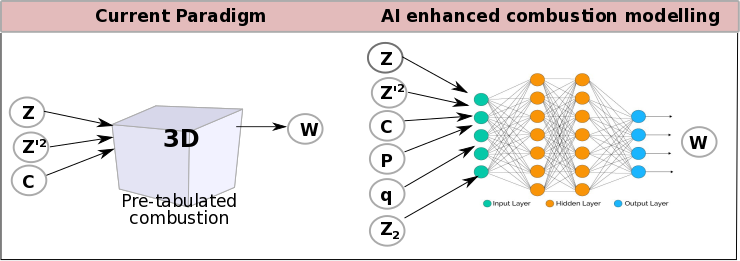
\includegraphics[width=\textwidth]{figs/AI_combustion.png}
\end{figure}
\end{frame}


\section{Concluding Remarks}
\begin{frame}{Conclusion}
\begin{itemize}
\item Multiphysics problems with supercritical flows encountered in many applications: energy production, nuclear engineering (SWCR), automotive engineering (diesel injection systems), aerospace propulsion
\end{itemize}
\end{frame}

\begin{frame}[c]{}
\begin{center}
{\LARGE{Thanks!}}\\
\vspace{0.8cm}

\url{jean-pierre.hickey@uwaterloo.ca}\\
\url{www.mpilab.ca}
\end{center}
\end{frame}

